%!TEX program = xelatex
\documentclass[a4paper,12pt]{report}
\usepackage{ctex}
%\usepackage{xeCJK}
\usepackage{times}
\usepackage{graphicx,float}
\usepackage{setspace}
\usepackage{fancyhdr}
% \usepackage{graphicx}
\usepackage{wrapfig}
\usepackage{array}
\usepackage{fontspec,xunicode,xltxtra}
\usepackage{titlesec}
\usepackage{titletoc}
\usepackage[titletoc]{appendix}
\usepackage[top=30mm,bottom=30mm,left=20mm,right=20mm]{geometry}
\usepackage{cite}
\usepackage{listings}
\usepackage{xcolor}
\usepackage{amsmath}
\usepackage{booktabs}
\lstset{
    basicstyle=\small\ttfamily, % 基本样式
    frame=single, % 代码块边框
    tabsize=4, % 制表符宽度
    numbers=left, % 行号位置
    language=Java, % 代码语言
    showstringspaces=false, % 不显示字符串中的空格
    commentstyle=\color{gray}, % 注释颜色
    keywordstyle=\color{blue}, % 关键字颜色
    stringstyle=\color{red}, % 字符串颜色
}
\usepackage[framed,numbered,autolinebreaks,useliterate]{mcode} % 插入代码
\XeTeXlinebreaklocale "zh"
\XeTeXlinebreakskip = 0pt plus 1pt minus 0.1pt

%---------------------------------------------------------------------
%	页眉页脚设置
%---------------------------------------------------------------------
\fancypagestyle{plain}{
	\pagestyle{fancy}      %改变章节首页页眉
}

\pagestyle{fancy}
\lhead{\kaishu~``人工智能物联网导论''实验报告~}
\rhead{\kaishu~~梁涵杰、李时玉、杨毅~~}
\cfoot{\thepage}

%---------------------------------------------------------------------
%	章节标题设置
%---------------------------------------------------------------------
%\titleformat{\section}{\centering\zihao{-1}\heiti}{报告\chinese{section}}{1em}{}
%\titlespacing{\section}{0pt}{*0}{*6}

%---------------------------------------------------------------------
%	摘要标题设置
%---------------------------------------------------------------------
\renewcommand{\contentsname}{\centerline{\zihao{2} 目\quad 录}}

%---------------------------------------------------------------------
%	参考文献设置
%---------------------------------------------------------------------
\renewcommand{\bibname}{\centerline{\zihao{2}{参\hspace{0.5em}考\hspace{0.5em}文\hspace{0.5em}献}}}

%---------------------------------------------------------------------
%	引用文献设置为上标
%---------------------------------------------------------------------
\makeatletter
\def\@cite#1#2{\textsuperscript{[{#1\if@tempswa , #2\fi}]}}
\makeatother

%---------------------------------------------------------------------
%	目录页设置
%---------------------------------------------------------------------
%\titlecontents{chapter}[0em]{\songti\zihao{-4}}{\thecontentslabel\ }{}
%{\hspace{.5em}\titlerule*[4pt]{$\cdot$}\contentspage}
%\titlecontents{section}[2em]{\vspace{0.1\baselineskip}\songti\zihao{-4}}{\thecontentslabel\ }{}
%{\hspace{.5em}\titlerule*[4pt]{$\cdot$}\contentspage}
%\titlecontents{subsection}[4em]{\vspace{0.1\baselineskip}\songti\zihao{-4}}{\thecontentslabel\ }{}
%{\hspace{.5em}\titlerule*[4pt]{$\cdot$}\contentspage}
\renewcommand\thesection{\arabic{section}}
\renewcommand\thesubsection{\arabic{section}.\arabic{subsection}}

\begin{document}


%---------------------------------------------------------------------
%	封面设置
%---------------------------------------------------------------------
\begin{titlepage}
	\begin{center}
		
    
\includegraphics[width=1.0\textwidth]{figure//nankai.jpg}\\
    % \vspace{10mm}
    % \textbf{\zihao{2}\kaishu{软件学院}}\\[0.8cm]
    \vspace{50mm}
    \textbf{\zihao{1}\heiti{ 《人工智能物联网导论》实验报告}}\\[3cm]
    \textbf{\zihao{2}\heiti{ Attention U-Net 图像分割}}\\[3cm]
	\vspace{\fill}
	
\setlength{\extrarowheight}{3mm}
{\songti\zihao{3}	
\begin{tabular}{rl}
	
	
{\makebox[4\ccwd][s]{组员 1:}}& ~\kaishu 梁涵杰 2120230780~~ \\

{\makebox[4\ccwd][s]{组员 3:}}& ~\kaishu 李时玉 2120230778~~ \\

{\makebox[4\ccwd][s]{组员 2:}}& ~\kaishu 杨 \ \ \ 毅 2120230799~~ \\


\end{tabular}
 }\\[2cm]
\vspace{\fill}
\zihao{4}
2023\textasciitilde 2024第二学期\\
	\end{center}	
\end{titlepage}


%---------------------------------------------------------------------
%  目录页
%---------------------------------------------------------------------
\tableofcontents % 生成目录

%---------------------------------------------------------------------
%
%---------------------------------------------------------------------
\newpage

\section{模型背景概述}

\subsection{U-Net}
U-Net 是一种基于卷积神经网络(CNN)的模型,最早由 Olaf Ronneberger 等人在 2015 年提出,专为生物医学图像分割设计。U-Net 的结构呈 U 形,包含一个编码器(encoder)和一个解码器(decoder)。U-Net 的关键特性在于其跳跃连接(skip connections),即将编码器每一层的特征图直接连接到相应解码器层。这种结构能够有效保留图像的细节信息,提高分割精度。

\begin{figure}[H]
    \centering
    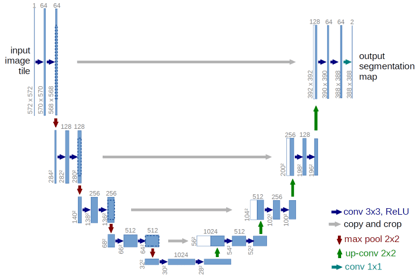
\includegraphics[width=0.8\textwidth]{figure/U-Net.png}
    \caption{U-Net}
    \label{fig:login}
\end{figure}


\subsection{注意力机制}
注意力机制起源于自然语言处理领域,旨在模拟人类视觉选择性注意的过程。通过为输入数据的不同部分分配不同的权重,注意力机制能够突出重要特征,抑制不相关信息。其主要类型包括:
\begin{itemize}
    \item 自注意力(Self-Attention):关注输入序列中各位置间的相关性。
    \item 注意力加权(Attention Weighting):为输入数据的各部分分配不同的权重。
\end{itemize}

\subsection{Attention U-Net}

Attention U-Net 是一种用于医学图像分割的深度学习模型,其主要在传统 U-Net 的基础上进行了改进,引入了注意力机制(Attention Mechanism)以增强模型的性能。

Attention U-Net 主要应用于医学图像分割任务,如肿瘤检测、器官分割等。由于其在保留细节和强调重要特征方面的优势,Attention U-Net 在许多医学图像分割任务中表现出色,显著提升了分割精度和鲁棒性。

\begin{figure}[H]
    \centering
    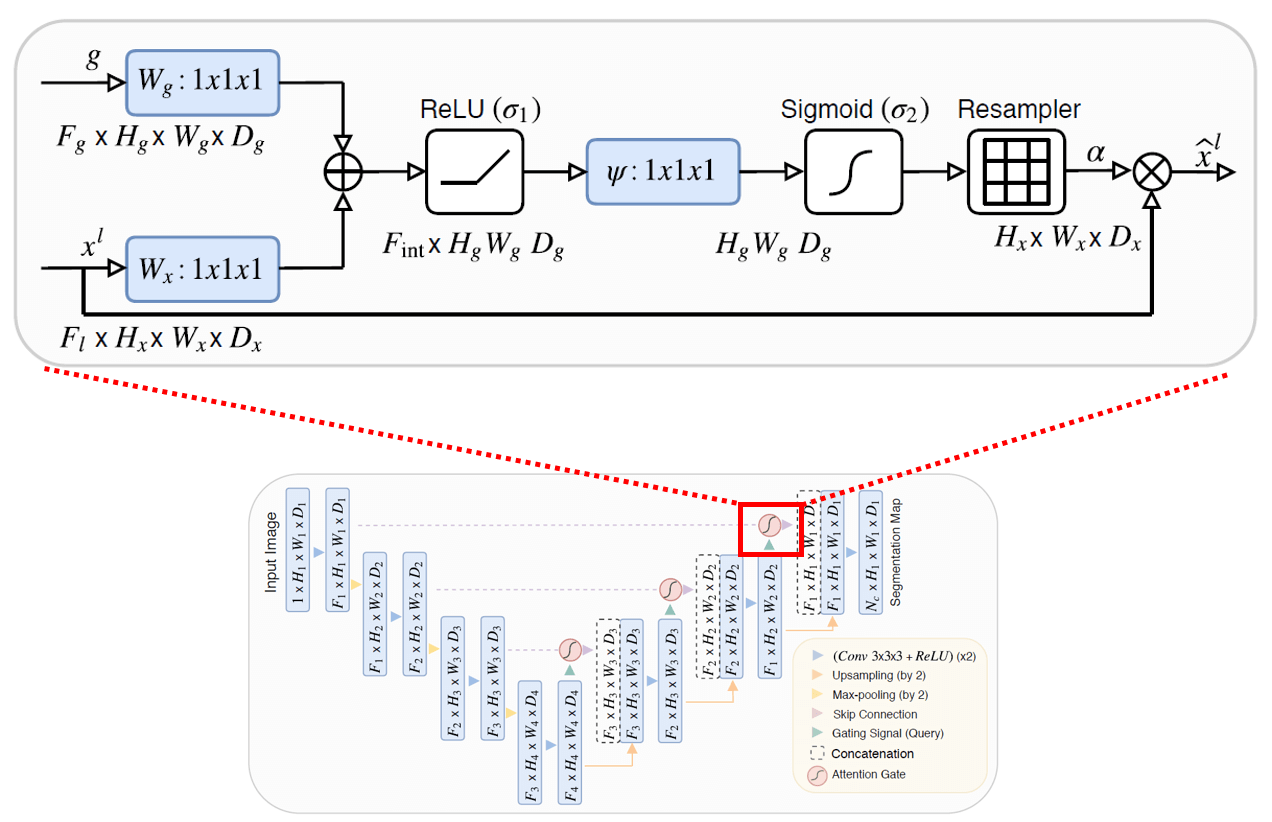
\includegraphics[width=0.8\textwidth]{figure/AttU-Net.png}
    \caption{Attention U-Net}
    \label{fig:login}
\end{figure}





\section{数据集介绍}
本实验使用提供的 Synapse 数据集,训练集大小为 2000 , 测试集大小为 1500。

\subsection{Synapse 数据集}
Synapse 数据集由腹部CT扫描图像组成,包含多个器官的手动标注。这些器官包括肝脏、脾脏、胰腺、肾脏和其他重要器官。Synapse 数据集是一个重要的医学图像分割数据集,广泛应用于多器官分割任务中。其高质量的图像和详细的器官标注为开发和评估分割模型提供了宝贵的资源,对于推动医学影像分析和相关技术的发展具有重要作用。

\subsection{数据集目录结构}
\begin{lstlisting}[language=Python]
Synapse/
  ├─ lists/
  │  └─ lists_Synapse/
  │     ├─ all.lst
  │     ├─ test_vol.txt
  │     └─ train.txt
  ├─ test_vol_h5/
  │  ├─ case0001.npy.h5
  │  ├─ case0002.npy.h5
  │  └─ ...
  └─ train_npz/
     ├─ case0005_slice000.npz
     ├─ case0005_slice001.npz
     └─ ...
\end{lstlisting}


\subsection{DataSet 类}

\begin{lstlisting}[language=Python]
class SynapseDataset(Dataset):
    def __init__(self, data_list, data_dir, transform=None):
        self.data_list = data_list
        self.data_dir = data_dir
        self.transform = transform

    def __len__(self):
        return len(self.data_list)

    def __getitem__(self, idx):
        file_name = self.data_list[idx]+''
        file_path = os.path.join(self.data_dir, file_name)
        # print(file_path)
        if file_path.endswith('.npz'):
            data = np.load(file_path)
            image = data['image']
            label = data['label']

        elif file_path.endswith('.h5'):
            with h5py.File(file_path, 'r') as f:
                images = np.array(f['image'])
                labels = np.array(f['label'])
                for img in images:
                    image = img

                for lab in labels:
                    label = lab

        else:
            raise ValueError("Unsupported file format")
        
        if self.transform:
            image, label = self.transform(image, label)
        
        image = torch.tensor(image, dtype=torch.float32).unsqueeze(0)  
        label = torch.tensor(label, dtype=torch.float32).unsqueeze(0)

        return image, label
\end{lstlisting}

\section{参数设置情况}
本网络模型基于 python3.8 和 pytorch1.9 实现。输入图像尺寸为512 × 512像素。在一张具有8 GB内存的Nvidia RTX 2070 GPU上训练U-net、Att-Unet、FCN模型。训练参数设置为:epoch为100,batch size为3,初始学习率为0.15,使用SGD(stochastic gradient descent)优化器(动量为0.9,权重衰减10-5)来优化反向传播模型。


\section{模型实验结果}
\subsection{评价指标}
采用Dice相似系数(Dice Similarity Coefficient,DSC)和交并比(Intersection over Union,IoU)作为评价指标,对当前模型的性能优劣进行全面评估。Dice相似系数特别强调图像分割中像素的内部填充,能够对模型的分割精度进行有效约束。而交并比则能衡量预测区域与真实区域之间的重叠程度。将DSC与IoU结合使用,不仅能够从不同角度反映模型的分割效果,还能相互补充,提高评估的全面性和准确性,从而有助于获得更加精确和可靠的分割结果。这种综合评价方法可以更全面地评价模型在图像分割任务上的表现,为进一步优化模型提供有力的指导。

\subsection{实验结果}

在Synapse数据集上,我们对三种不同的图像分割方法进行了实验,分别是FCN、U-Net和Attention U-Net。实验数据如下表所示:

\begin{table}[H]
    \centering
    \begin{tabular}{ccccc}
         \toprule %[2pt]
         方法 & Train Dice & Train Iou & Val Dice & Val Iou\\
         \midrule %[2pt]
         FCN & 0.56 & 0.55 & 0.39 & 0.34\\
         U-Net & 0.57 & 0.56 & 0.45 & 0.41\\
         Attention U-Net & 0.57 & 0.55 & 0.47 & 0.43\\
         \bottomrule %[2pt]
    \end{tabular}
    \caption{不同方法在Synapse数据集上的分割精度}
\end{table}



\begin{figure}[H]
    \centering
    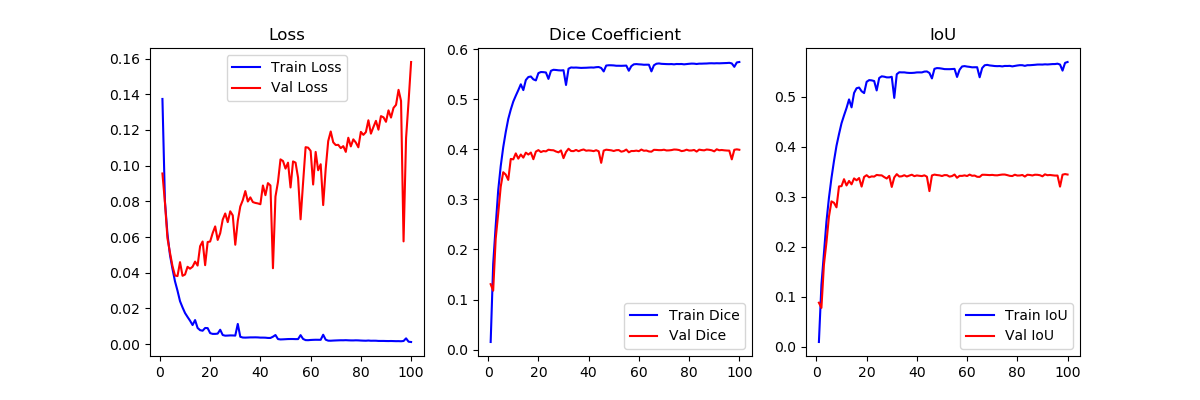
\includegraphics[width=0.8\textwidth]{figure/FCNtraining_metrics_epochs_100.png}
    \caption{FCN}
    \label{fig:login}
\end{figure}

\begin{figure}[H]
    \centering
    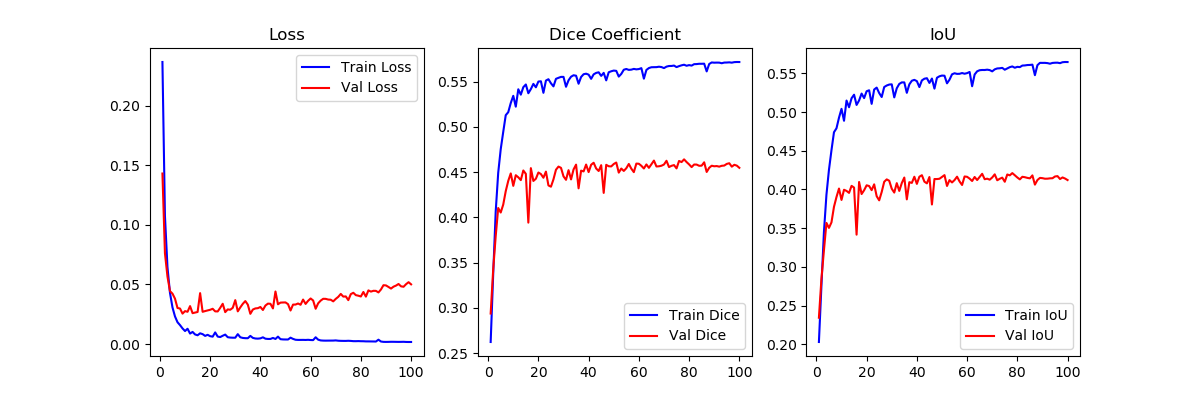
\includegraphics[width=0.8\textwidth]{figure/UNettraining_metrics_epochs_100.png}
    \caption{U-Net}
    \label{fig:login}
\end{figure}

\begin{figure}[H]
    \centering
    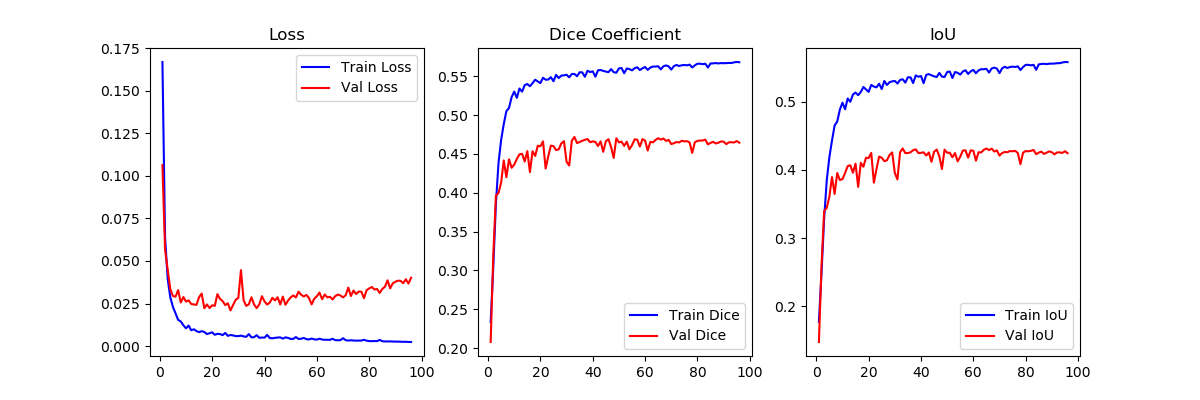
\includegraphics[width=0.8\textwidth]{figure/AttU_Net_training_metrics_epochs_96.png}
    \caption{Attention U-Net}
    \label{fig:login}
\end{figure}

\section{相关分析和结论}

\subsection{结果分析}
\begin{itemize}
    \item \textbf{训练集表现}:
        \begin{itemize}
            \item FCN在训练集上的Dice系数和IoU分别为0.56和0.55,表现较为稳定。
            \item U-Net的训练集表现稍优于FCN,Dice系数为0.57,IoU为0.56。
            \item Attention U-Net的训练集表现与U-Net相似,Dice系数为0.57,IoU为0.55。
        \end{itemize}
    \item \textbf{验证集表现}:
        \begin{itemize}
            \item 在验证集上,FCN的表现最差,Dice系数为0.39,IoU为0.34。
            \item U-Net在验证集上的表现明显优于FCN,Dice系数为0.45,IoU为0.41。
            \item Attention U-Net在验证集上的表现最好,Dice系数为0.47,IoU为0.43。
        \end{itemize}
\end{itemize}

\subsection{结论}
从实验结果可以看出,Attention U-Net在Synapse数据集上的整体表现最好,其验证集上的Dice系数和IoU均高于其他两种方法。具体分析如下:

\begin{itemize}
    \item \textbf{FCN}:
        \begin{itemize}
            \item 在训练集和验证集上的表现均较差,特别是在验证集上的表现远低于其他两种方法,说明其泛化能力较弱。
        \end{itemize}
    \item \textbf{U-Net}:
        \begin{itemize}
            \item 在训练集和验证集上的表现均好于FCN,特别是在验证集上的提升明显,说明U-Net较好地捕捉到了数据的特征,具有较强的泛化能力。
        \end{itemize}
    \item \textbf{Attention U-Net}:
        \begin{itemize}
            \item 在训练集上的表现与U-Net相似,但在验证集上的表现最好,说明引入注意力机制后,模型能够更有效地关注重要的特征区域,提高了分割精度。
        \end{itemize}
\end{itemize}

\section{相关问题和解决方法}

\subsection{问题: 测试数据集加载异常}
实验中编写 dataset 类构建数据集时,使用相同的方式构建了训练集和测试集中的数据,在训练过程中发现训练集中的数据正常,但是测试集中的张量出现4个维度[1,89,512,512]不符合预期,在检查代码后发现由于测试集中的一个文件中包含了多组image 和label,所以出现了异常的数据。

\subsection{解决方法}
重新编写了 dataset 类,在读取测试集的时候,预先读取每一个文件中的images和labels,存到数组中,再进行处理,代码实现如下:
\begin{lstlisting}[language=Python]
class SynapseDataset_test(Dataset):
    def __init__(self, data_list, data_dir, transform=None):
        self.data_list = data_list
        self.data_dir = data_dir
        self.transform = transform
        # self.resize = transforms.Resize((512, 512))
        self.data_list_len = len(self.data_list)

        self.images =[]
        self.labels =[]
        

        for idx in range(self.data_list_len):
            file_name = self.data_list[idx]+''
            file_path = os.path.join(self.data_dir, file_name)
            # print(file_path)

            with h5py.File(file_path, 'r') as f:
                images = np.array(f['image'])
                labels = np.array(f['label'])
                for img in images:
                    self.images.append(img)

                for lab in labels:
                    self.labels.append(lab)

    def __len__(self):
        return len(self.images)

    def __getitem__(self, idx):
        image = self.images[idx]
        label = self.labels[idx]

        image = torch.tensor(image, dtype=torch.float32).unsqueeze(0)  # Add channel dimension
        label = torch.tensor(label, dtype=torch.float32).unsqueeze(0) 
        # print("image_size:{} , label_size:{}".format(image.shape,label.shape))
        
        return image, label
\end{lstlisting}


\section{小组成员分工描述和占比}
\begin{itemize}
    \item 梁涵杰(33.3\%) :数据集处理、模型训练、文档编写
    \item 李时玉(33.3\%) : FCN 模型构建、模型测试评估、文档编写
    \item 杨毅  (33.3\%) : U-Net 模型构建、Attention U-Net 模型构建、文档编写
\end{itemize}


\end{document}
